% !TEX root = ~/OpenFOAM/antoniopucciarelli-9/run/LABS/thermochemical_CFD/main.tex

% INCOMPRESSIBLE CASE 
\section{Incompressible flow - $\mathtt{Lab02}$}

    \renewcommand{\thepage}{\arabic{page}}
    \setcounter{page}{\thelastPage}

All the properties relative to the incompressible flow solvers - \verb|SIMPLE|, \verb|PISO| and \verb|PIMPLE| - are described in detail in~\ref{app:app1}. 

%\subsection{$t$ discretization in OpenFOAM}
%In \verb|PISO/PIMPLE| the time advancing is made in order to discretize the time derivative. As result, the $t$ advancing in the \verb|PISO/PIMPLE| solver has a physical meaning. The contrary is for the \verb|SIMPLE| solver where, in the \verb|fvSchemes|, the time discretization is absent (Listing~\ref{list:ddtSchemes}). In \verb|SIMPLE|, the $t$ advancement is essentially a controller for an additional loop over the predictor-corrector steps. As result, the previous step gives us a better estimate of $p^* - \boldsymbol{u}^*$ used for the numerical problem assembly.

%\begin{lstlisting}[caption = $\mathtt{combustorSimple/system/fvSchemes}$ time discretization., label = list:ddtSchemes]
%ddtSchemes  // time derivative discretization 
%    {       // no need of temporal discretization in SIMPLE algorithm
%        default steadyState; // => no time stencil 
%    }
%\end{lstlisting}

%\cprotect\subsection{\verb|PISO| vs \verb|PIMPLE|}
%The main difference between these two models consists in the \textbf{outer} correction. \verb|PISO| does not have outer correctors. The outer corrector loop consists in a correction of $p^* - \boldsymbol{u}^*$ used in the predictor step\cprotect\footnote{Solved if \verb|momentumPredictor yes;| in \verb|applications/solvers/incompressible/simpleFoam| with check on \verb|simple.momentumPredictor()|.}. This allows, relating all the process to the $\boldsymbol{u}$ at the previous outer corrector step, to find a much more correct estimate of $\boldsymbol{u}$ at the new time step due to the fact that we have a better system formulation (based on $p - \boldsymbol{u}$ already estimated at the end of the previous predictor-corrector steps) that makes the problem treatment much like an \textbf{implicit} method. The \textbf{outer} correction step is very computational demanding but, at the same time, it is possible using $\Delta t$ such that $Co > 1$. So choosing between \verb|PISO| and \verb|PIMPLE|, other than convergence and numerics, can be described with time step iterations\cprotect\footnote{It is important to keep in mind that \verb|pisoFoam| in OpenFOAM does not change the $\Delta t$. In order to solve this issue - so keeping $Co < 1$ and allowing $\Delta t$ to change -, it is used running \verb|pimpleFoam| in \verb|PISO| mode. Of course, the number of outer corrector for \verb|pimpleFoam| in \verb|PISO| mode is $0$.}.  

%\subsubsection{Courant-Friedrichs-Lewy} 
%In time marching problems, the CFL test allows to find a proper time step in order to link the \textbf{spatial} stencil with the \textbf{temporal} stencil, Figure~\ref{fig:CFL}.

%\begin{figure}[h!]
\vspace*{-1.5cm}
\centering
\definecolor{ttttff}{rgb}{0.2,0.2,1}
\definecolor{qqqqff}{rgb}{0,0,1}
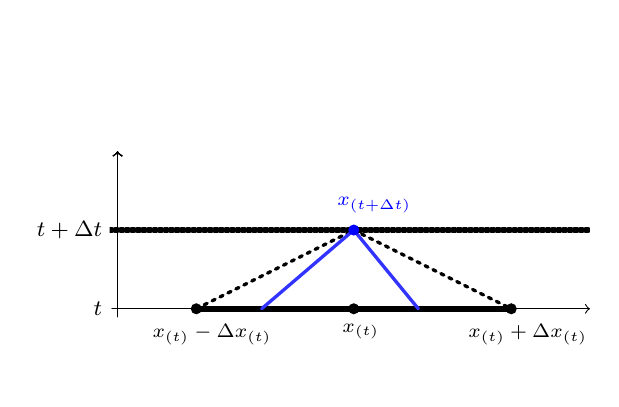
\begin{tikzpicture}[line cap=round,line join=round,x=1cm,y=1cm]
\draw[->,color=black] (1,0) -- (7,0);
\foreach \x in {1,2,3,4,5,6,7}
\draw[->,color=black] (1,-0.1) -- (1,2);
\draw[shift={(1,0)},color=black] (2pt,0pt) -- (-2pt,0pt) node[left] {\footnotesize ${t}$};
\draw[shift={(1,1)},color=black] (2pt,0pt) -- (-2pt,0pt) node[left] {\footnotesize $t + \Delta t$};
\clip(0.9,-0.89) rectangle (7,3.57);
\draw [line width=2pt,dash pattern=on 1pt off 1pt,domain=-0.37:7.9] plot(\x,{(--4-0*\x)/4});
\draw [line width=2pt] (2,0)-- (4,0);
\draw [line width=2pt] (4,0)-- (6,0);
\draw [line width=1.2pt,dotted] (2,0)-- (4,1);
\draw [line width=1.2pt,dotted] (4,1)-- (6,0);
\draw [line width=1.2pt,color=ttttff] (4,1)-- (4.82,0);
\draw [line width=1.2pt,color=ttttff] (4,1)-- (2.83,0);
\begin{scriptsize}
\fill [color=black] (2,0) circle (2pt);
    \draw[color=black] (2.2,-0.1) node[below] {$x_{(t)} - \Delta x_{(t)}$};
\fill [color=black] (4,0) circle (2pt);
    \draw[color=black] (4.09,-0.09) node[below] {$x_{(t)}$};
\fill [color=black] (6,0) circle (2pt);
    \draw[color=black] (6.21,-0.1) node[below] {$x_{(t)} + \Delta x_{(t)}$};
\fill [color=qqqqff] (4,1) circle (2pt);
    \draw[color=qqqqff] (4.26,1.12) node[above] {$x_{(t + \Delta t)}$};
\end{scriptsize}
\end{tikzpicture}
    
    \caption{CFL, spatial and temporal stencils.}
    \label{fig:CFL}

\end{figure}


%As result, it is ensured that the $p - \boldsymbol{u}$ fields are physically related to the previous time steps. Of course, using $Co < 1$ does not guarantee achieving convergence; the convergence is related also to the discretization schemes and the correctors - so mainly, how the problem is solved -. The CFL condition is expressed as \cite[Ch. 13]{quarteroni2012numerical}:

%\begin{equation}
%    max_{\Omega} \Bigg( \frac{\big| \boldsymbol{u} \big| \ \Delta t}{\Delta x} \Bigg) < 1.0
%    \label{eqn:CFL}
%\end{equation}

%\noindent From (\ref{eqn:CFL}), $\Delta t$ is computed. There are methods, such as \verb|PIMPLE|, that allow relaxation on this stencils constraint; this is mainly related to the way the solution is computed. $Co > 1$ acts as a filter on the solution: physics with time scales shorter than $\Delta t$ are not seen in the final solution e.g. vortex shedding. In addition, for $Co > 1$ the time discretization error propagates on the solution; the last time step is the initial condition for the new time step. In OpenFOAM the Courant-Friedrichs-Lewy conditions is expressed through \verb|maxCo|. 

%\subsection{Under relaxation}
%The under relaxation consists in changing the value of a computed field in order to smooth out convergence. The under relaxation process followed in many codes is the \textbf{Patankar} model~\cite[Ch. 14.1]{moukalled2016finite}, that consists in an explicit (\ref{eqn:expPATANKAR}) and an implicit (\ref{eqn:PATANKAR}) formulation:
%\begin{align}
%    \phi_{j + 1}^{relaxed} & = \phi_{j} + \alpha_{\phi} \ \big( \phi_{j + 1} - \phi_{j} \big) \label{eqn:expPATANKAR} \\ 
%    \frac{a_C}{\lambda_{\phi}} \ \phi_{C_{j + 1}} + \sum_F a_F \ \phi_{F_{j + 1}} & = b_C + \frac{1 - \lambda_{\phi}}{\lambda_{\phi}} \ a_C \ \phi_{C_j} 
%    \label{eqn:PATANKAR}
%\end{align}

%\noindent This model relies on $\alpha_{\phi}$ that is the relaxation parameter of the $\phi$ field. The most used $\alpha_{\phi}$ values are: $\alpha_{\boldsymbol{u}} \approx 0.7$ and $\alpha_{p} \approx 0.3$. Now, having explained the relaxation model, it is necessary to relate it to the different algorithms. The under relaxation is not present in the \verb|PISO| algorithm; this because the under relaxed field without outer corrector loop generates a not physical field, so it should not became an output of the solver. As this said, the \verb|PISO| algorithm outputs directly the $p$ field and the corrected $\boldsymbol{u}$ field ($\boldsymbol{u} = \boldsymbol{u}_{(p, \ \boldsymbol{u}^*)}$). The other algorithms, \verb|SIMPLE| and \verb|PIMPLE|, allow using under relaxation. The under relaxation parameters are expressed in \verb|system/fvSolution| with \verb|relaxationFactors| and it can be explicit on a field with \verb|fields| setting or implicit in the equations with \verb|equations| setting.

\subsection{Problem setup}
\subsubsection{Boundary conditions}
The boundary conditions to be set are relative to the $p-\boldsymbol{u}$ and the turbulence model. Since the problem is incompressible, $p$ is expressed as $\frac{p}{\rho}$ in order to facilitate the computation\cprotect\footnote{This brings to set the \verb|p| boundary conditions dictionary \verb|dimensions [0 2 -2 0 0 0 0];|.}. The internal field for $p-\boldsymbol{u}$ is $0$. 

\paragraph{Turbulence model}
Since the \verb|RAS| model uses the $\kappa-\varepsilon$ tubulence model~\cite[Ch. 10.4]{pope2000turbulent}, set in \verb|constant| with \verb|momentumTransport|, it is needed to set up $\kappa-\varepsilon-\nu_t$ boundary conditions. 

\subparagraph{$\varepsilon$} For $\varepsilon$ (turbulent dissipation rate $\frac{1}{2} \ \nu < s_{ij}^{\prime} s_{ij}^{\prime} >$\footnote{$s_{ij}^{\prime} = \frac{1}{2} \big( \frac{\partial u_i^{\prime}}{\partial x_j}  + \frac{\partial u_j^{\prime}}{\partial x_i} \big)$, deviatoric part of $\boldsymbol{\nabla \ u}^{\prime} $}), the inlets have the same turbulence setup \verb|turbulentMixingLengthDissipationRateInlet| and the \verb|mixingLength| is fixed\footnote{Key parameter for the computation of $\nu_t$.}. The walls are modeled with a wall function model: \verb|epsilonWallFunction|. The outlet is set to \verb|zeroGradient| (it means that $\varepsilon$ does not change \textbf{in space} at the outlet). 

\subparagraph{$\kappa$} The $\kappa$ (turbulent kinetic energy $\sum_i < u_i^{\prime} u_i^{\prime} >$) follows the same philosophy of $\varepsilon$ - turbulent model at the inlet with \verb|turbulentIntensityKineticEnergyInlet|, \verb|kqrWallFunction| at the wall and \verb|zeroGradient| at the outlet -.

\subparagraph{$\nu_t$} Although $\nu_t$ (turbulent viscosity to be added to the molecular viscosity $\nu$ described in \verb|constant/transportProperties|) is completelly described by $\kappa-\varepsilon$, it is possible to impose boundary conditions on it. $\nu_t$ at the walls is modelled with a wall function model \verb|nutkWallFunction|; the rest of the field is directly computed via $\kappa-\varepsilon$ model.  

\subsubsection{Schemes}
\cprotect\paragraph{\verb|fvSchemes|} All the fields are discretized with a second order interpolation based on Gauss integration. The laplacian field and the surface normal gradient schemes are set to \verb|corrected| that means the non orthogonality property is corrected via correctors (that allows sticking with a second order accuracy model).  

\cprotect\paragraph{\verb|fvSolution|}
In the unsteady solver it is described the number of outer correctors, \verb|nOuterCorrectors|, and the number of internal correctors, \verb|nCorrectors|\cprotect\footnote{\verb|nNonOrthogonalCorrectors 0;| because the mesh has low non orthogonality.}. Turbulence is set as present in all the outer correctors with \verb|turbOnFinalIterOnly no;|, this allows to have a better evaluation of $\nu_t$. It is set the relaxation factors only for \verb|combustorPimpleCFL15| in order to guarantee convergence due to \verb|maxCo 15;|. In \verb|combustorPimpeCFL1| there are not present any relaxation factors, this partially because \verb|maxCo 1;| that allows less changes of the solution over the time steps. The \verb|combustorPimple1| set up is not like \verb|PISO| because there are $100$ outer correctors (\verb|PISO| has none). 

For the error check it has been used \verb|tolerance| and \verb|relTol| both in the iterative methods, used for the computation of the fields, and also on the outer correctors (that can be seen as a refinement process of the $p^* - \boldsymbol{u}^*$ variables). Solvers are based on \verb|GAMG|\footnote{Generalised geometric algebraic multi grid: used for the momentum equation solution (asymmetric matrix).} and \verb|smoothSolver|\cprotect\footnote{Solver that uses a smoother: in the cases it is used for the continuity equation - Poisson equation - (symmetric matrix). Of course the smoother model has to be described with \verb|smoothSolver|.}. In the \verb|combustorPimpleCFL15|, the \verb|*Final|\cprotect\footnote{This is a way of treating differently the last outer corrector cycle. The last outer corrector cycle depends on \verb|nOuterCorrectors| or if the outer corrector tolerances are satisfied.} relative tolerances (\verb|relTol|) are set to $0$; this in order to guarantee convergence using an error check based on \verb|tolerance|. 

\subsection{Post processing}
The post processing functions are declared in \verb|system/controlDict|. The main values extracted are the solution's initial residuals, the forces on the splitter, the $y^+$ in the boundarly layer close to the walls and the $U_y$ velocity at $y = 100 mm$. 

\subsection{Results}
\cprotect\subsubsection{\verb|combustorSimple|}
It is possible to see that \verb|simpleFoam| does not reach convergence. This is a \textbf{numerical error} related to the body geoemtry: it is a bluff body. As result the solution oscillates between 2 \textit{numerical} admissible solutions. The point here is that it is trying to simulate an unsteady phenomena with a steady solver. 

There are not problems with the drag force computation. Since the geometry is symmetric, the drag force over the \textit{fitious} time steps is the same. 

\cprotect\subsubsection{\verb|combustorPimpleCFL1|}
With \verb|maxCo 1;| constraint, the results represent the vortex shedding after the splitter. Since the non physical initial conditions, the drag force has a large escursion the first time steps but then it settles down to a constant value. This constant value of drag force is made by the low changing pressure field around the splitter, although the vortex shedding in time. 

\cprotect\subsubsection{\verb|combustorPimpleCFL15|}
With \verb|max Co 15;| constraint, in this case the vortex shedding phenomena starts to show later in the solution. This is related to the filtering action of using a stable - outer corrector - solver with unlinked time-space discretization. As in the other solvers, the first time steps are affected by large escursion in the drag force due to the convergence of the internal field.  

\newpage

% PAGE MANAGEMENT
% saving page number
%\newcounter{lastPage}
%\addtocounter{lastPage}{\thepage}
\setcounter{lastPage}{\thepage}
% changing page numbering for the results figures
\setcounter{page}{1}
\renewcommand{\thepage}{INC-\roman{page}}

\begin{figure}[!h]
    \centering
    \import{latexFIGS/lab02/}{residuals.pgf}
    \caption{Incompressible cases: residuals.}
    \label{fig:Res}
\end{figure}

\begin{figure}[!h]
    \centering
    \import{latexFIGS/lab02/}{Uy.pgf}
    \caption{Incompressible cases: $U_y$.}
    \label{fig:Uy}
\end{figure}

\begin{figure}[!h]
    \centering
    \import{latexFIGS/lab02/}{forces.pgf}
    \caption{Incompressible cases: forces.}
    \label{fig:forces}
\end{figure}

\begin{figure}[!h]
    \centering
    \import{latexFIGS/lab02/}{yPlus.pgf}
    \caption{Incompressible cases: $y^+$.}
    \label{fig:yPlus}
\end{figure}

\begin{figure}[!h]
    \includegraphics[width=\textwidth]{latexFIGS/figs/combustorPimple15.png}
    \caption{Velocity profile for combustor with CFL < 15.}
\end{figure}

\clearpage
